
\documentclass[tikz,border=5mm]{standalone}
\usetikzlibrary{decorations.pathreplacing}
\begin{document}

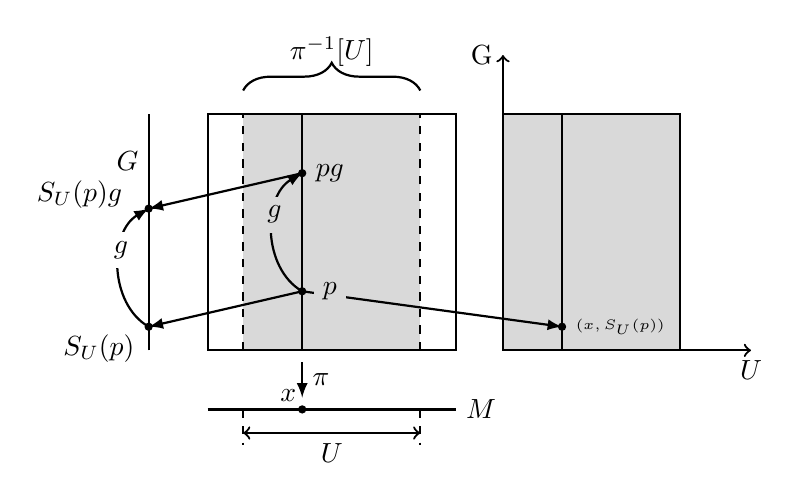
\begin{tikzpicture}[scale=1.5]

% Colors and shaded regions
\fill[gray!30] (0,0) rectangle (1.5,2); % Left rectangle
\fill[gray!30] (2.2,0) rectangle (3.7,2); % Right rectangle

% Outlines of rectangles
 \draw[thick] (-0.3,0) rectangle (1.8,2); % Left rectangle outline
 \draw[thick] (2.2,0) rectangle (3.7,2); % Right rectangle outline
 \draw[dashed, thick] (0,0) -- (0,2);
  \draw[dashed,thick] (1.5,0) --(1.5,2);
  \draw[thick] (0.5,0) -- (0.5,2);
  \draw[thick] (2.7,0) -- (2.7,2);
  \draw[thick] (-0.3,-0.5) -- (1.8,-0.5) node[right] {$M$};
  \draw[thick,->] (2.2,0) -- (2.2,2.5) node[left] {G};
  \draw[thick,->] (2.2,0) -- (4.3,0) node[below] {$U$};
  \draw[thick] (-0.8,0) -- (-0.8,2) node[pos = 0.8,left]{$G$};

  \draw[thick ,-latex] (0.5,0.5) to[out = 150, in = -150] (0.5,1.5) node[fill = gray!30,xshift = -10,yshift = -15]{$g$};
\draw[thick ,-latex] (-0.8,0.2) to[out = 150, in = -150] (-0.8,1.2)node[fill = white,xshift = -10,yshift = -15]{$g$};
\draw[dashed,thick] (0,-0.5) -- (0,-0.8);
\draw[dashed,thick] (1.5,-0.5) -- (1.5,-0.8);
\draw[thick,<->] (0,-0.7) -- (1.5,-0.7) node[pos = 0.5,below]{$U$} ;
\draw[decorate, decoration={brace, amplitude=10pt}, thick] (0,2.2) -- (1.5,2.2)node[midway, above, yshift=5pt] {$\pi^{-1}[U]$};
\draw[thick,-latex] (0.5,-0.1)--(0.5,-0.4) node[pos = 0.5,right] {$\pi$};
\draw[thick,-latex] (0.5,0.5) -- (-0.8,0.2);
\draw[thick,-latex] (0.5,1.5) -- (-0.8,1.2);
\draw[thick,-latex] (0.5,0.5) -- (2.7,0.2);
\fill (0.5,0.5) circle (1pt) node[fill = gray!30,xshift = 10]{$p$};
\fill (0.5,1.5) circle (1pt) node[fill = gray!30,xshift = 10]{$pg$};
\fill (-0.8,0.2) circle (1pt)node[fill = white,xshift = -18,yshift = -8]{$S_U(p)$};
\fill (-0.8,1.2) circle (1pt)node[fill = white,xshift = -25,yshift = 5]{$S_U(p)g$};
\fill (2.7,0.2) circle (1pt) node[fill = gray!30,xshift = 21,font=\tiny]{$(x,S_U(p))$};
\fill (0.5,-0.5) circle (1pt) node[xshift = -5,yshift = 5 ] {$x$};
\end{tikzpicture}

\end{document}
